%%% Dateikodierung: UTF-8
%%% äöüÄÖÜß  <-- keine deutschen Umlaute hier? UTF-faehigen Editor verwenden!

%%% Magic Comments zum Setzen der korrekten Parameter in kompatiblen IDEs
% !TeX encoding = utf8
% !TeX program = pdflatex 
% !TeX spellcheck = de_DE
% !BIB program = biber

\documentclass[internship,german,smartquotes]{hgbthesis}
% Zulässige Optionen in [..]: 
%    Typ der Arbeit: 'diploma', 'master' (default), 'bachelor', 'internship' 
%    Hauptsprache: 'german' (default), 'english'
%    Option zur Umwandlung in typografische Anführungszeichen: 'smartquotes'
%    APA Zitierstil: 'apa'
%%%-----------------------------------------------------------------------------

\RequirePackage[utf8]{inputenc} % bei Verw. von lualatex oder xelatex entfernen!

\graphicspath{{images/}}  % Verzeichnis mit Bildern und Grafiken
\logofile{logo}           % Logo-Datei: images/logo.pdf (kein Logo: \logofile{})
\bibliography{references} % Biblatex-Literaturdatei (references.bib)

%%%-----------------------------------------------------------------------------
% Angaben für die Titelei (Titelseite, Erklärung etc.)
%%%-----------------------------------------------------------------------------

% \title{toya\\ Imperative Programmiersprache für die JVM}
% \author{Lukas Christian Hofwimmer}
% \programname{Universal Computing}

%\programtype{Fachhochschul-Bachelorstudiengang} % auswählen/editieren
% \programtype{Fachhochschul-Bachelorstudiengang}

% \placeofstudy{Hagenberg}
% \dateofsubmission{2021}{07}{15} % {YYYY}{MM}{DD}

% \advisor{FH-Prof. DI Dr. Heinz Dobler} % optional

%\strictlicense % restriktive Lizenz anstatt Creative Commons (nicht empfohlen!)

%%%-----------------------------------------------------------------------------
\begin{document}
%%%-----------------------------------------------------------------------------

%%%-----------------------------------------------------------------------------
\frontmatter                                       % Titelei (röm. Seitenzahlen)
%%%-----------------------------------------------------------------------------

% \maketitle
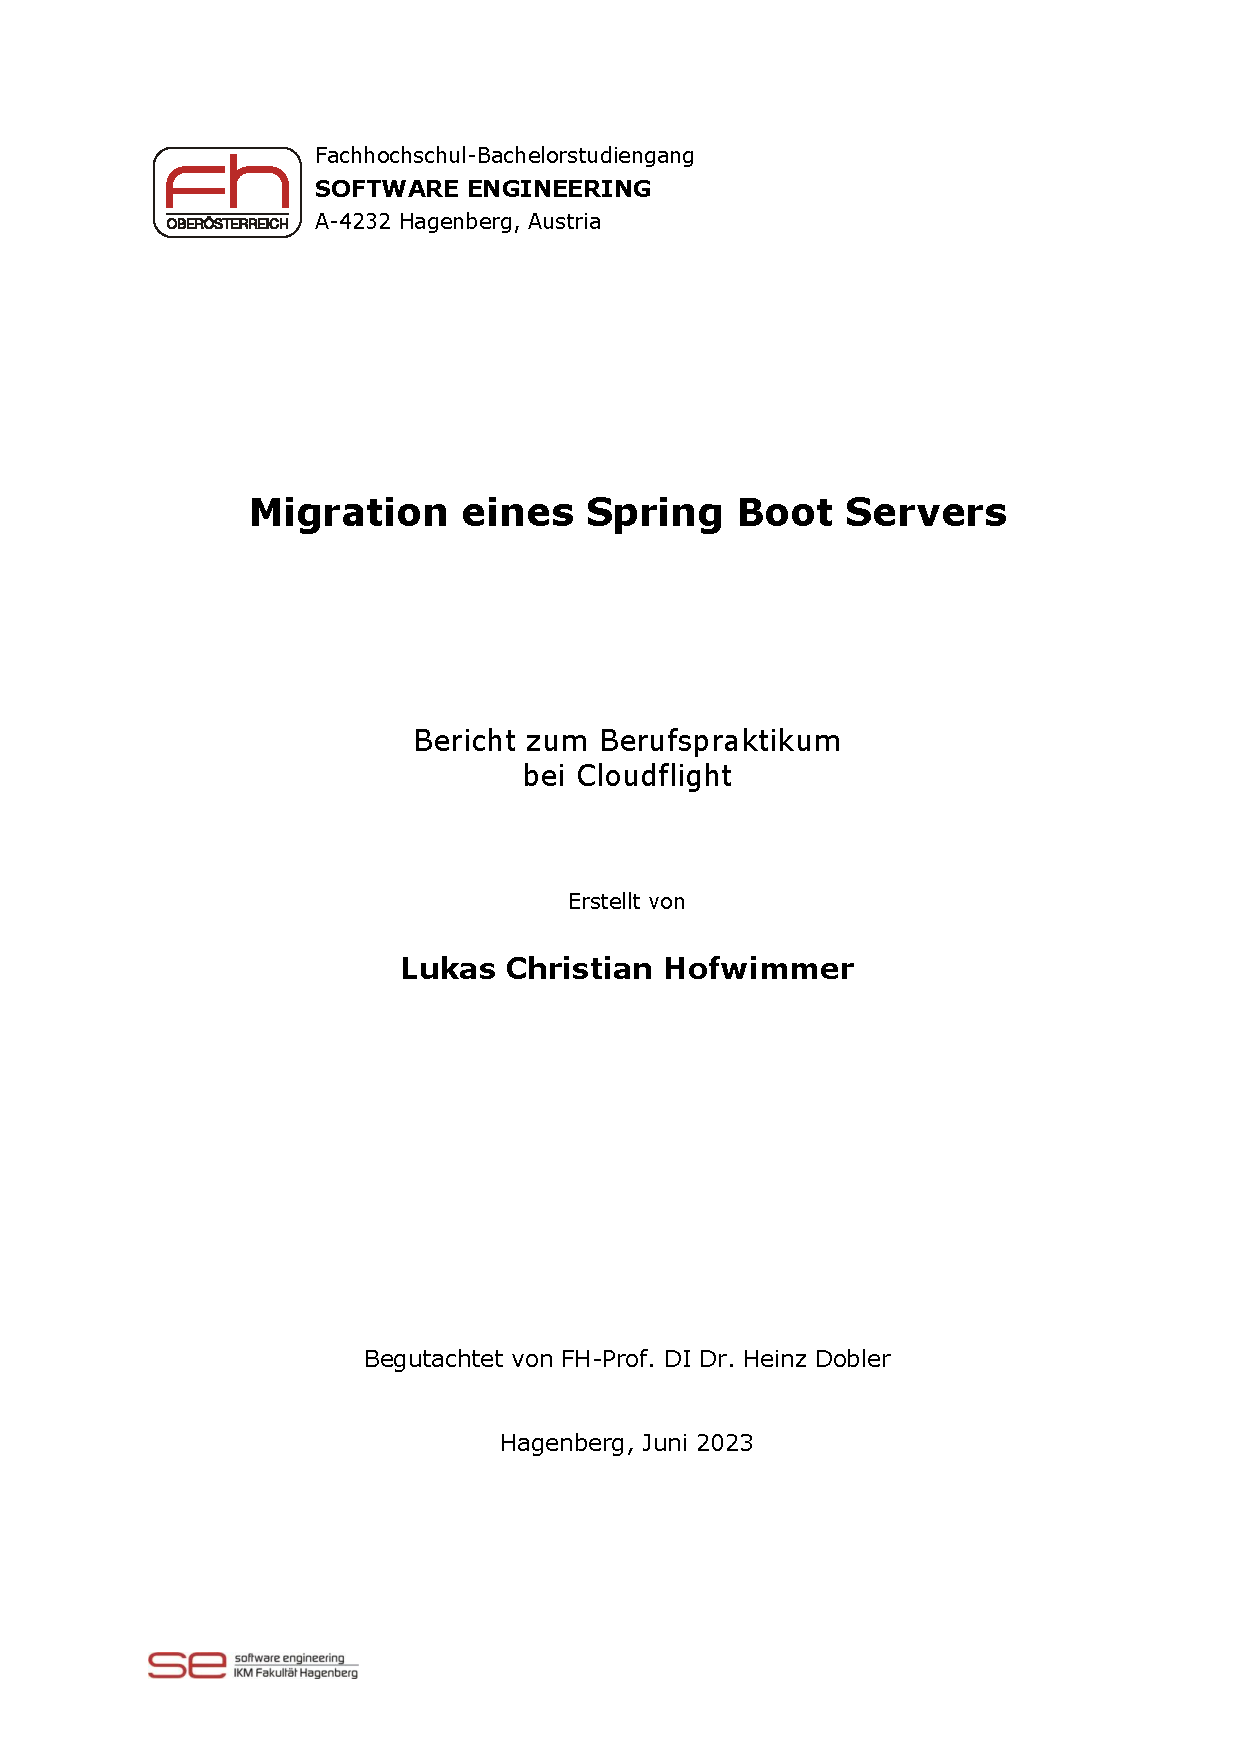
\includepdf[pages=1, pagecommand={\thispagestyle{empty}}]{Titelblatt_BP.pdf}
\tableofcontents

\chapter{Kurzfassung}

		
\chapter{Abstract}

			

%%%-----------------------------------------------------------------------------
\mainmatter                             % Hauptteil (ab hier arab. Seitenzahlen)
%%%-----------------------------------------------------------------------------

\chapter{Einleitung}
\label{cha:intro}

Im Zuges des Berufspraktikums im sechsten Semester durfte ich mein Können als Software-Entwickler bei der Firma Cloudflight beweisen. Dabei konnte ich viele wertvolle Erfahrungen und Eindrücke mitnehmen, mein Fachwissen verbessern und ein praktisches Verständniss dafür entwickeln, wie man eine Firma dieser Größenordnung richtig leitet und organisiert. 

\section{Cloudflight}

Cloudflight ist ein Linzer IT-Unternehmen. Es wurde 2005 unter dem Namen Catalysts von Christoph Steindl und Christian Federspiel in Linz gegründet und spezialisiert sich auf Dienstleistungs-Software für Drittunternehmen. Das Unternehmen besteht aus einer Vielzahl von kleinere Teams, die sich jeweils um ein Projekt kümmern. Dadurch kann eine Vielzahl an verschiedenen Kunden gleichzeitig betreut werden. Auftraggeber reichen von privaten Firmen wie Fronius bis hin zu staatlichen Insitutionen, wie das Land Oberösterreich oder die europäische Raumfahrtsbehörde.

Ein besonderes Augenmerk ist auf den alle sechs Monate stattfindenden CCC - \textit{Cloudflight Coding Contest} zu legen. Dabei veranstaltet Cloudflight an einer Vielzahl von europäischen Bildungseinrichtungen einen Wettkampf, bei dem es unter Zuhilfenahme von Programmierung gilt, immer herausforderndere Rätsel zu lösen.

\section{Zielsetzung}

Die Hauptaufgabe des Praktikums besteht darin, das \textit{Customerportal} von Spring Boot 2 auf Spring Boot 3 zu aktualisieren. Was sich auf den ersten Blick als banale Aufgabe darstellt, entpuppt sich jedoch im Laufe dieser Arbeit als Rhizom-artige Struktur, die ein komplexes Abhängigkeitsgeflecht darstellt. 

Dabei gilt es, nicht nur eine bloße Aktualisierung von Spring Boot selbst durchzuführen, sondern auch Bibliotheken, wie den Code-Generator und den Dokumentations-Generator auf einen neuen Stand zu bringen.

Zusätzlich, aber mit einer niedrigeren Priorität, muss auch das Frontend in Form einer Angular Web-Applikation aktualisiert werden. Original entwickelt wurde das \textit{Customerportal} 2020, seither aber nicht am aktuellsten Stand gehalten.

\section{Nebenaufgaben}

Neben der Hauptaufgabe um Spring Boot wurden auch kleinere Nebenaufgaben erledigt. Die beiden größten dabei waren die Aktualisierung der Android-Applikation \textit{mathe2go} und das Schreiben von Dokumentation bezüglich der Verwendung von \textit{Structurizr}. 

\subsection{mathe2go}

\textit{mathe2go} ist eine Android- und iOS-Applikation zur Unterstützung von Schülern in der Vorbereitung auf die Zentralmatura in Mathematik. Schüler loggen sich in der App ein, lernen Theorieabschnitte - in Kapitel eingeteilt- und prüfen dieses Wissen anschließend in \textit{Quicktests} und einem Abschlusstest ab. Original stammt dieses Projekt aus 2017. Dieses Projekt diente zusätzlich als Einstiegsprojekt meines Praktikums, da es ein kleineres Projekt in Umfang war.

Google fordert, dass Apps im Google Play Store mit neuen Android Versionen kompatibel bleiben muss. Kommen nun Deprecations einer Api in einer neuen Android Version hinzu, müssen Anpassungen im Code vorgenommen werden, dass es zu keinen Problemen bei Endnutzern kommt. Nach mehreren Jahren der Instandhaltung kamen einige größere Punkte, die bisher unerledigt blieben, zusammen und konnten auf einmal behandelt werden. So wurde von der Bibliothek \texttt{Butterknife} zum nativen Ansatz mit Viewbindings gewechselt, die Bibliothek zum lokalen Caching durch \texttt{sqldelight} ersetzt und einige Unit-Tests und Integrations-Tests geschrieben.

\subsection{Structurizr}

Die zweitere - kleinere - Nebenaufgabe dreht sich um \textit{Structurizr} und das C4 Modell. Konkret ist \textit{Structurizr} eine Web-Applikation zum Erstellen, Generieren und Bearbeiten von C4 Modellen. C4 Modelle sind der Versuch, den Gedanken hinter UML-Diagrammen auf gesamte Software-Systeme zu übertragen und standardisieren. Software-Systeme sind in vier Schichten unterteilt. Diese sind wie folgt:

\begin{enumerate}
    \item \textbf{System Context} stellt die höchste und damit auch die abstrakteste Schicht des Modells dar. Hier interagieren die Benutzer mit dem System. Der Fokus liegt darauf, ein Software-System und dessen Kontext im umliegenden Feld darzustellen. Mögliche \textit{System Contexts} sind zum Beispiel ein Email-System. Das zentrale Backend eines Systems.
    \item \textbf{Container} konkretisieren ein Software-System, sind aber weiterhin sehr abstrakt. Mögliche Container sind eine Angular-Applikation, die Datenbank, das Backend.
    \item \textbf{Components} umfassen Teile eines Containers. Das umfasst zum Beispiel eine Login-Komponente oder das Authentifizierungs-System im Backend.
    \item \textbf{Code} ist die detailierteste Ebene im C4 Modell. Hier liegt Code im Form eines UML-Diagrammes.
\end{enumerate}

Bisher bestand die Firmen-interne Dokumentation für \textit{Structurizr} nur sehr fragmentiert. Daher wurde im Umfang dieses Praktikums auch eine Aufbereitung vorgenommen und eine detailierte Anleitung zur Verwendung von \textit{Structurizr} erstellt. Dabei gibt es zwei Ansätze zur Erstellung des C4 Modells: manuell und automatisch in Form einer Compiler-Erweiterung. Beide diese Ansätze wurden dokumentiert und im zentralen Wissensspeicher der Firma gespeichert.

\section{Struktur der Arbeit}

Dieser Bericht ist in vier Kapitel unterteilt. Die \nameref{cha:intro} beschreibt kurz das Unternehmen und kleinere Nebenaufgaben, die während des Praktikums erledigt wurden. Außerdem entählt es die Zielsetzung der Hauptaufgabe und eine Übersicht über die Struktur. 
Im Kapitel \nameref{cha:design} geht dieser Bericht auf die Ausgangslage, den Projektkontext, verwendete Technologien und Lösungsansätze ein und erklärt das \textit{Customerportal} im Detail. \nameref{cha:implementation} zeigt die praktische Umsetzung der Migration auf Spring Boot 3 und wie das Ergebnis auf dessen Funktionalität getestet wurde. Das Kapitel \nameref{cha:synopsis} schildert persönliche Erfahrungen des Autors und welche Schritte im weiteren Verlauf zu erledigen wären.
\chapter{Konzept}
\label{cha:design}

Dieses Kapitel beschreibt den theoretischen Kontext und notwendige Überlegungen, um im Kapitel \nameref{cha:implementation} die Migration problemlos umsetzen zu können. Außerdem erläutert es den nötigen Kontext, um die notwendigen Änderungen des \textit{Customerportals} nachvollziehen zu können. Namentlich handelt es sich dabei um firmeninterne Bibliotheken, die zentrale Komponenten des Systems darstellen. Ebenso zeigt es den Status Quo vor dem Projektstart und den organisatorischen Kontext.

\section{Customerportal}

Das \textit{Customerportal} ist eine 2020 entwickelte Plattform, die Firmen beim Versand von Push-Benachrichtigungen unterstützt. Benutzer:innen können Zielgruppen verwalten, Inhalte für Push-Nachrichten erstellen und bearbeiten und das Versenden dieser automatisieren. Mithilfe der \texttt{CampaignSender} Bibliothek ist es möglich, plattformunabhängig Nutzer zu benachrichtigen. Die unterstützten Plattformen belaufen sich auf iOS, Android und Google Chrome. Das Herzstück des \textit{Customerportals} ist die Oberfläche zum Orchestrieren von Push-Benachrichtigungen. Dieser Prozess ist in drei Teile unterteilt:

\begin{enumerate}
    \item \textbf{Inhalt:} Hier wählt die Nutzer:in einen Titel und den textuellen Inhalt für die zu erstellende Push-Benachrichtigung aus. Optional kann der Inhalt auch aus einer Liste von bereits erstellten Vorlagen ausgewählt werden. Inhalte können auch mit Platzhaltern versehen werden, um Nachrichten durch die Verwendung von Namen zum Beispiel zu personalisieren. Zusätzlich besteht noch die Möglichkeit, das Verhalten beim Klick auf die Benachrichtigung zu steuern. So lässt sich nicht nur die App öffnen, sondern auch gezielt auf bestimmte Unterseiten verweisen, dass zum Beispiel ein bestimmter Nachrichtenartikel geöffnet wird. Pro Plattform können beliebig viele \textit{Actions} definiert werden.
    \item \textbf{Zielgruppe:} Dieser Schritt erlaubt das Auswählen und Einschränken einer Zielgruppe. Zielgruppen können zuerst aus einer Liste von Zielgruppen ausgewählt werden. Das Erstellen neuer Einträge dieser Liste ist über den Import von CSV-Dateien möglich. Jede Person einer Zielgruppe besitzt einige Metadaten, wie zum Beispiel Sprache oder Plattform. Anhand dieser Metakriterien ist es möglich, die Zielgruppe einzuschränken. Benutzer:innen von \textit{Customerportal} ist es möglich, eigens definierte Filterkriterien anzulegen. Wünscht Resch\&Frisch etwa, dass ein neues Filterkriterium \textit{Glutenunverträglichkeit} notwendig ist, kann dieses leicht hinzugefügt werden.
    \item \textbf{Sendeverhalten:} Hier ist es abschließend noch möglich, das Absendeverhalten zu konkretisieren. Push-Benachrichtigungen können entweder sofort, zu einem fixen Zeitpunkt in der Zukunft oder in regelmäßigen Intervallen auf täglicher oder wöchentlicher Basis versendet werden.
\end{enumerate}

Das \textit{Customerportal} kann entweder selbst betrieben oder als von \textit{Cloudflight} betrieben SaaS-Lösung verwendet werden. \textit{Cloudflight} bietet zur Basis-Applikation noch Zusatzmodule, die den Funktionsumfang erweitern. Zu den Kunden des \textit{Customerportals} zählen unter anderem Resch\&Frisch, Linz AG und Abfall OÖ. 

Original unter \textit{mogree} entwickelt, ging das \textit{Customerportal} 2022 mit dem Verkauf von \textit{mogree} an \textit{Cloudflight} automatisch auch in deren Besitz über. Seit der originalen Entwicklungsarbeit 2020 wurden kaum Instandhaltungsmaßnahmen daran vorgenommen, was sich nunmehr drei Jahre später zeigt. Schwerwiegende Sicherheitslücken wie CVE-2021-44228 (\textit{Log4Shell}) wurden seither entdeckt und stellen ein fortbestehendes Sicherheitsrisiko dar~\parencite{cvelog4shell}. Mit 2023 gilt es nun, eine aktualisierte Version des \textit{Customerportals} zu erstellen.

\section{Projektkontext}

Der Startschuss für dieses Projekt wurde mit der dritten Woche des Berufspraktikums angesetzt, nachdem die bisherige Aufgabe des \textit{mathe2go} Projektes abgeschlossen werden konnten. Die Abnahme der geleisteten Arbeit erfolgt durch den Vorgesetzten Andreas Schweiger, der auch schon 2020 technische Führungskraft war.

Große Teile der Arbeit wurden auf selbstständiger Basis erledigt. Bei Pull-Requests und technischen Diskussionen erfolgte die Zusammenarbeit mit dem Kollegen Johannes Krenn, der momentan nebenberuflich zum Master-Studium an der FH Hagenberg noch bei Cloudflight tätig ist.

\section{Projektarchitektur}

Das zentrale System des Customerportals ist das Backend in Form einer Spring Boot Applikation. Das Backend stellt eine REST-Api zur Verfügung. Der Zugriff darauf ist entweder durch die REST-Api direkt oder mit dem Angular Frontend als Benutzeroberfläche möglich. Zusätzlich sind viele Funktionen und Mechanismen auf eigens entwickelte Bibliotheken ausgelagert.~\autoref{fig:c4-cp} zeigt das C4-Modell der Komponenten des \textit{Customerportals}.

\begin{figure}[h]
    \caption{C4-Modell des \textit{Customerportals}}
    \centering
    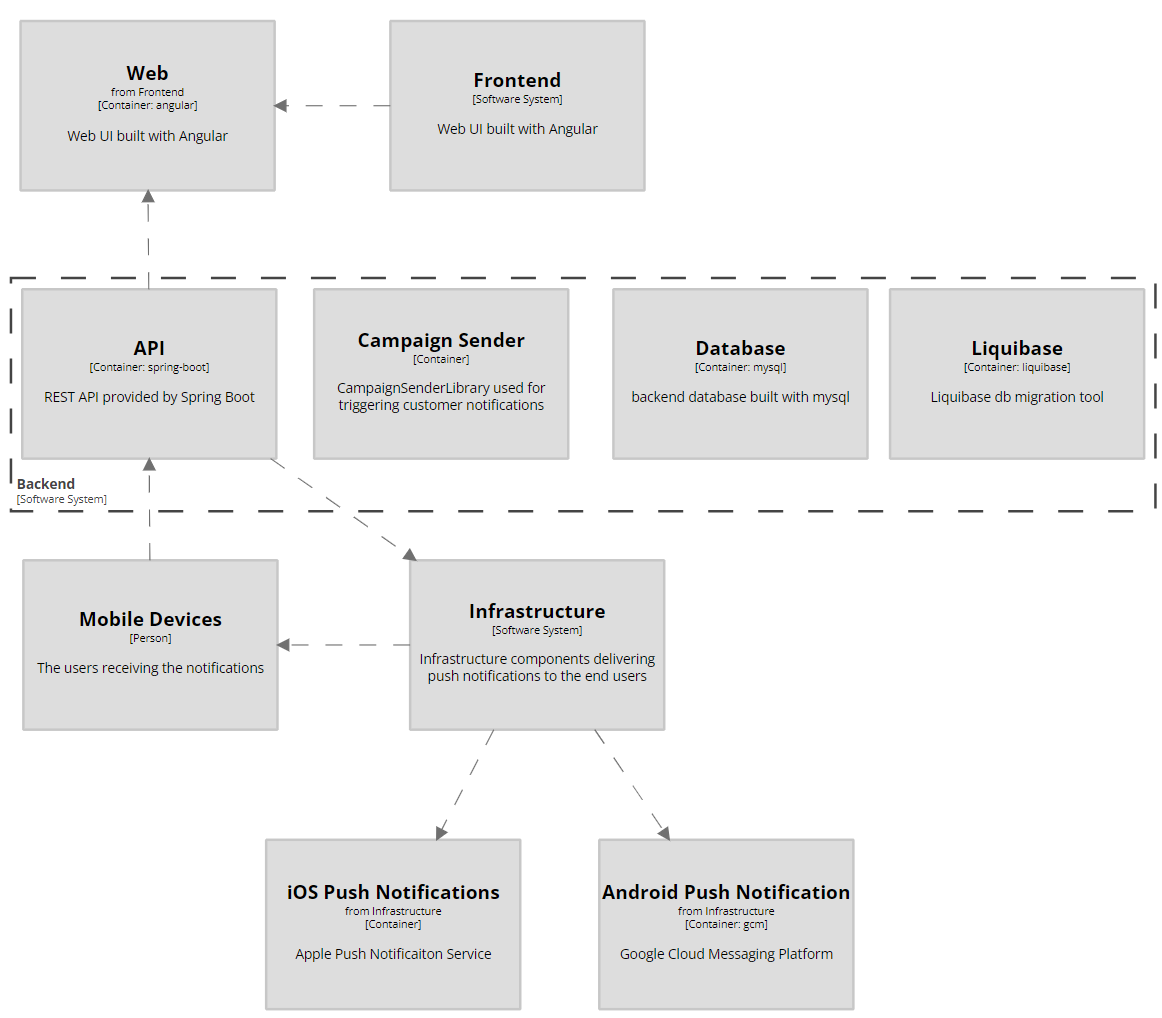
\includegraphics[width=\textwidth]{C4.Architecture.System}
    \label{fig:c4-cp}
\end{figure}

\subsection{Backend}

Das Backend umfasst mehrere wichtige Komponenten mit einer Spring Boot-Applikation im Zentrum. Dieses Backend stellt eine REST-Api zur Verfügung und nutzt OAuth2.0 zum Authentifizieren von Nutzern und zum Autorisieren von Zugriffen auf die Schnittstelle. Clients authentifizieren sich durch die Präsenz eines \texttt{Authorization}-Headers in der Http-Anfrage. Diesen Header erhält ein Client nach dem erfolgreichen Anmelden.

Eine MySql Instanz dient zum Persistieren der Daten. Liquibase wendet Migrationen auf die Datenbank an und befüllt diese mit Test-Daten, wenn es im Kontext einer Test-Umgebung ausgeführt wird. Sowohl die lokale Mysql-, als auch die Liquibase-Instanz laufen in Docker-Containern, die von einem Docker-Compose-Script orchestriert werden.

Benutzer und deren personenbezogene Daten werden verschlüsselt in der Datenbank gespeichert. Dadurch ist keine Nachverfolgung von bestimmten Nutzern möglich, sollte etwa ein Datenleck auftreten. Jedoch ist weiterhin die Anwendung von Filtern, wie zum Beispiel die Einschränkung der Altersgruppe möglich. 

Lokal wird das Backend typischerweise mit Intellij IDEA ausgeführt. Dasselbe gilt auch für die JUnit-Tests. Alternative kann das Customerportal jedoch auch containerisiert ausgeführt werden. Dadurch kann die Infrastruktur des Produktionssystem lokal simuliert werden.

Wichtige Teile des Backends sind auf private Bibliotheken, die mit Artifactory verwaltet werden, ausgelagert. Allen voran \texttt{mogree-codegen} zum Erzeugen der REST-Api. Die Bibliothek erzeugt auf Basis einer Spezifikation in einer Swagger-konformen yaml-Datei die Klassen der Schnittstelle. Dadurch muss nur die Logik eines Endpunktes in einem \texttt{Service} definiert werden. Meta-Informationen, wie zum Beispiel Swagger-Annotationen generiert die Bibliothek auf Basis der Spezifikationsdatei. Zum Erzeugen der REST-Api Quelldateien verwendet \texttt{mogree-codegen} \texttt{mustache}-Dateien als Schablone: Statische Textstücke sind direkt in der Datei enthalten. Variable Textfragmente, die sich je nach Endpunkt unterscheiden, haben im Text einen Platzalter (doppelte geschwungene Klammer - wie Angular). Bei der Übersetzung erzeugt die Bibliothek ein Modell, anhand welchem die Platzhalter durch Werte der Variablen ersetzt werden.

Ist zum Beispiel in einer Datei \texttt{swagger.yml} ein Endpunkt \texttt{/account/login} spezifiziert, wird die Schnittstelle \texttt{AccountDelegate} und die Klasse \texttt{AccountController} erzeugt. Beide Typen enthalten eine Funktion \texttt{login}. Der/Die Entwickler:in muss nun eine Klasse \texttt{AccountService} definieren, die \texttt{AccountDelegate} implementiert. Zusätzlich noch wird die Implementierung durch \texttt{@Component} zu einer injezierbaren Komponente in Spring und mit \texttt{@Primary} als Hauptimplementierung der Schnittstelle markiert. Die Klasse \texttt{AccountController} erhält nun die Implementierung der Delegateklasse aufgrund der Dependency-Injection-Mechanismen von Spring. Fehlercodes, wie zum Beispiel 401 (Unauthorized) werden durch Ausnahmezustände repräsentiert. Das Diagramm~\autoref{fig:codegen-diagram} zeigt diesen Prozess. \texttt{Mogree-codegen} erzeugt die folgenden vier Pakete:

\begin{itemize}
    \item \texttt{api}: Hier liegen die Controller der REST-Api. Jeder Controller implementiert eine Schnittstelle, die den Suffix -Api trägt und die Swagger-Annotationen enthält. Außerdem befindet sich hier der Delegate des Controllers .
    \item \texttt{config}: Hier liegt die Konfiguration der Swagger-UI.
    \item \texttt{model}: Dieses Paket enthält die DTOs, die an den Client zurückgesendet werden.
    \item \texttt{param}: Hier liegen die Param-Objekte, die an die Delegate-Implementierungen übergeben werden.
\end{itemize}

\texttt{Mogree-codegen} ist ein \textit{fork} der Bibliothek~\textcite{githubswaggercodegen}, da sie nicht alle Anforderungen erfüllte. Wie in~\autoref{lst:account_rest} zu sehen ist, erzeugt die \texttt{login}-Methode auf Basis der Parameter ein Objekt des Typs \texttt{ParamLogin} und übergibt es an die Implementierung des Delegates. Diese Param-Objekte werden in \texttt{swagger-codegen} nicht erzeugt, wodurch dieser \textit{fork} nötig war. Auf die Nachteile des selbst entwickelten Ansatzes geht dieser Bericht im weiteren Verlauf noch ein.

\begin{JavaCode}[numbers=none, caption={Der generierte \texttt{AccountController}}, label=lst:account_rest]
@RestController
public class AccountController implements AccountApi {
    ...
    public ResponseEntity<DetailResponse<UserAuthModel>> login(
            @Parameter(description = "Email of user", required = true)
            @RequestHeader(value = "mogree-Mail", required = true)
            String mogreeMail,
            @Parameter(description = "Password of user", required = true)
            @RequestHeader(value = "mogree-Password", required = true)
            String mogreePassword
    ) {
        ParamLogin paramLogin = new ParamLogin(mogreeMail, mogreePassword);
        return new Executer(validators).validate().usecase(() -> delegate.login(paramLogin)).run();
    }
}
\end{JavaCode}

Die Konfiguration des Zielverzeichnisses, des Vorlagenverzeichnisses und der Spezifikationsdatei erfolgt durch Gradle in der \textit{Task} \texttt{codegenConfig}. Diese \textit{Task} erfolgt in der Ausführungsphase von Gradle und wird dadurch bei jeder Kompilation ausgeführt~\parencite{gradlelifecycle}.

\begin{figure}[h]
    \caption{Ablauf der Codegenerierung anhand des Beispiels des AccountControllers.}
    \centering
    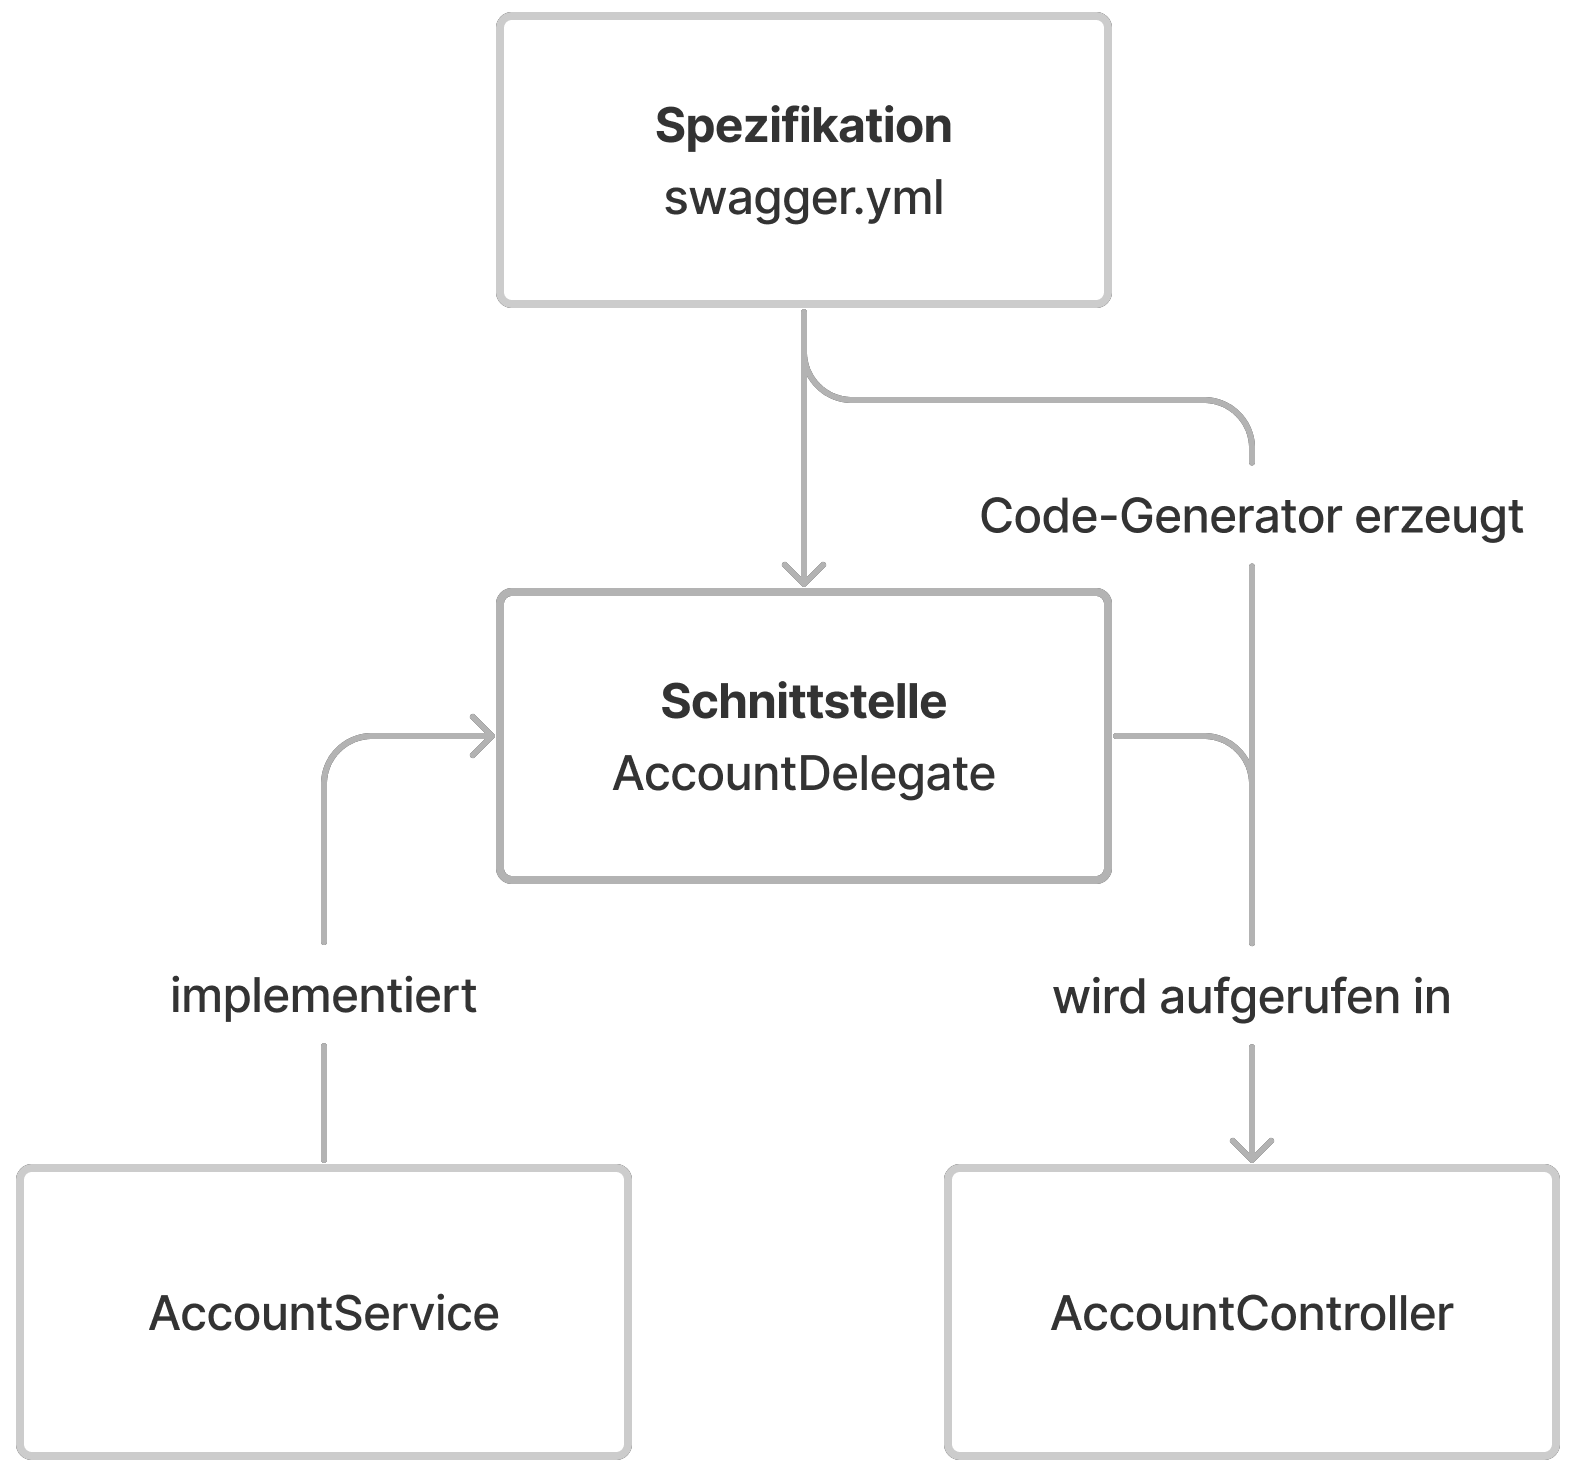
\includegraphics[scale=0.4]{Code.Generator}
    \label{fig:codegen-diagram}
\end{figure}

Neben \texttt{mogree-codegen} kommen noch weitere Bibliotheken zum Einsatz. Die Bibliothek \texttt{mogree-spring} bietet in vielen Teilbereichen von Spring Erweiterungen und Verbesserungen. So sind die \texttt{Validators}, die in~\autoref{lst:account_rest} zu sehen sind, in der Bibliothek enthalten. Ebenso werden auch viele Klassen und Schnittstellen, die bei der Verarbeitung von Client-Anfragen benötigt werden über \texttt{mogree-spring} bereitgestellt.

Die Bibliothek \texttt{library-jwt} enthält die Authentifizierungs- und Autorisierungslogik. Wie bereits erwähnt wird hierfür OAuth2.0 mit JWT verwendet. Außerdem übernimmt die Bibliothek die Einordnung der Autorisierungs-Filterregeln in der Spring \texttt{HttpSecurity}-Filterkette. Sollte im Autorisierungsprozess ein Ausnahmezustand auftreten, so übernimmt \texttt{library-jwt} die Behandlung davon.

Das Backend verwendet die Bibliothek \texttt{springfox} zum Bereitstellen der Swagger-UI. Swagger-UI dient zum Visualisieren der REST-Api. Die Benutzeroberfläche dafür ist unter dem Pfad \texttt{/api/v1/swagger-ui.html} im Browser verfügbar. Damit können Anfragen an den Server getätigt werden und die Antwort betrachtet werden.

\subsection{Frontend}
\label{sec:design-frontend}

Das Frontend ist eine Weboberfläche, die mit dem Framework Angular implementiert ist. Sie greift auf das Backend durch die Api zu. Die Komponenten der Benutzeroberfläche bauen auf Angular-Material-Komponenten auf, wobei teilweise Style-Änderungen vorgenommen wurden.~\autoref{fig:cp-web-home} zeigt die Startseite des Frontends.

\begin{figure}[h]
    \caption{Die Startseite des Customerportal-Frontends, die der/die Benutzer:in nach dem Login zu sehen bekommen.}
    \centering
    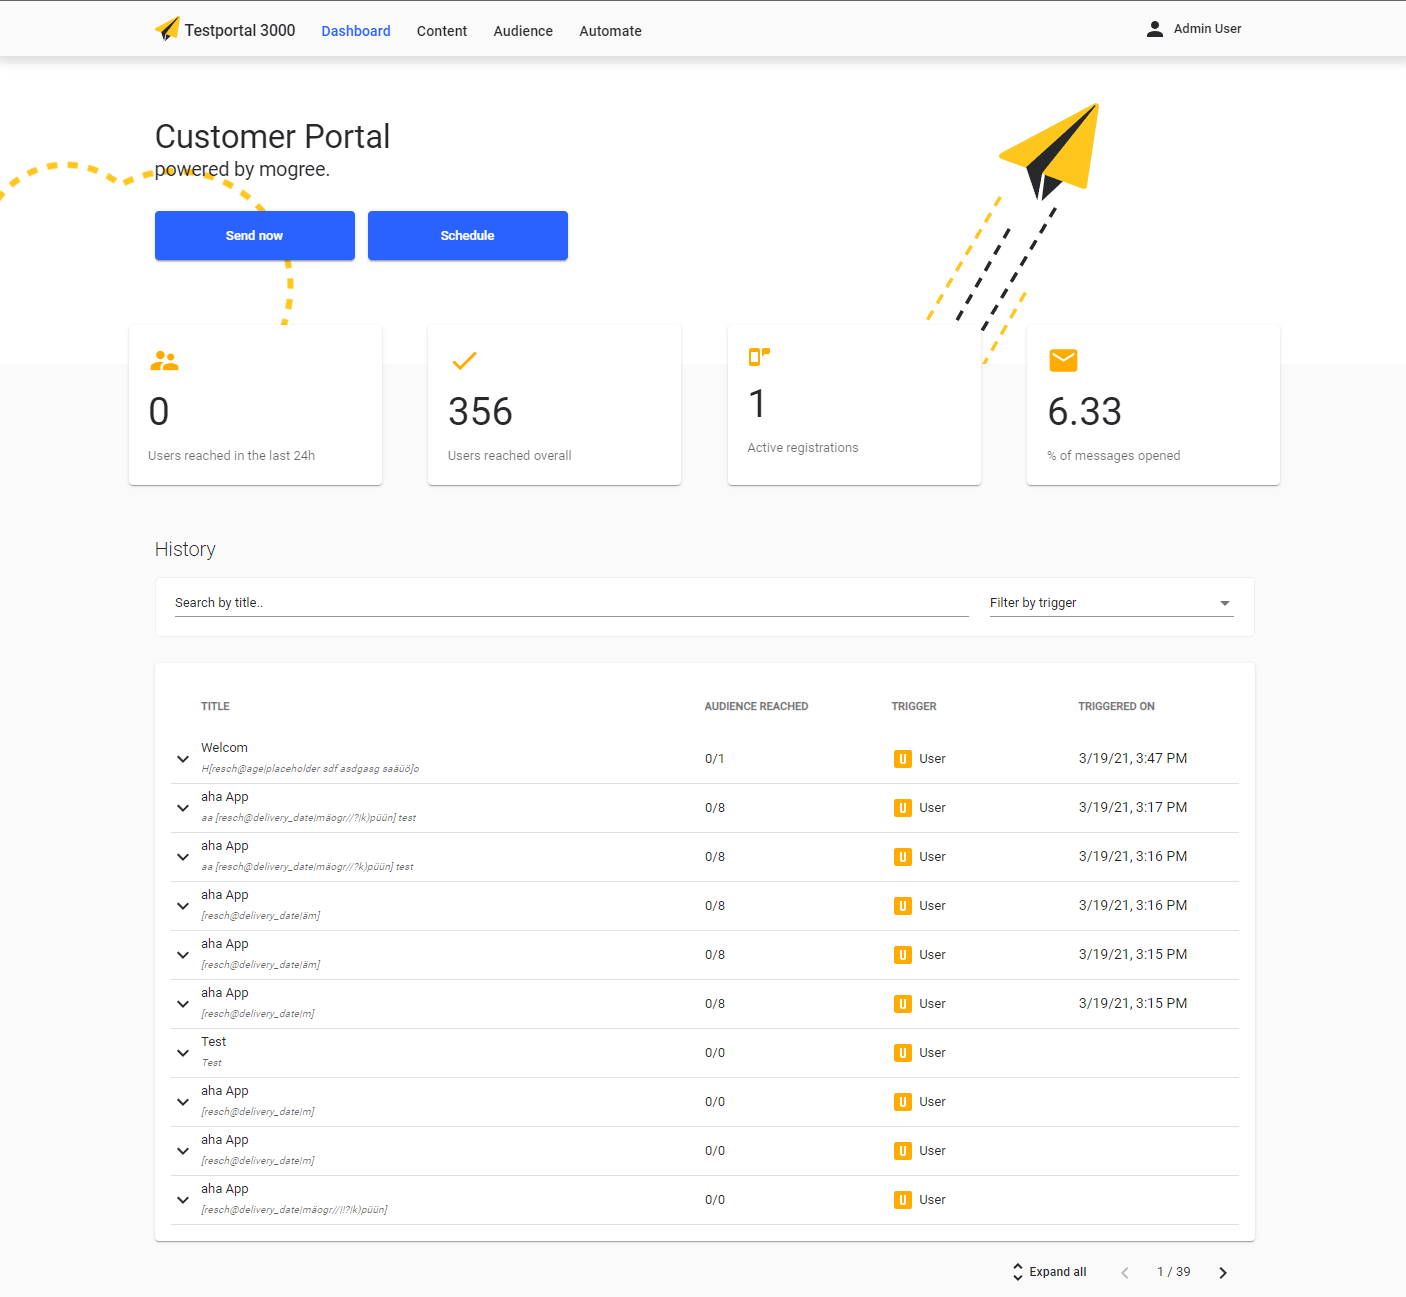
\includegraphics[scale=0.38]{CP.Web.Home}
    \label{fig:cp-web-home}
\end{figure}

Programmatisch ist das Frontend in einem desolaten Zustand. Viel Code ist hier schlecht geschrieben und sollte überarbeitet werden. Vor allem sind Komponenten oft viel zu groß. Teilweise überschreiten Viewmodel-Klassen die 1000-Zeilen Hürde. In solchen Fällen wäre eine Aufspaltung in mehrere kleinere Komponenten ratsam. Dadurch erhöht sich die Wiederverwendbarkeit und Lesbarkeit des Systems.

Der Codequalität ist auch auf der Mikro-Ebene schlecht. Funktionslogik hat oft eine höhere Komplexität als nötwendig oder sinnvoll. Teilweise sind Funktionen über 300 Zeilen lang und haben eine dreistellige zyklomatische Komplexität. 

\subsection{Infrastruktur}

Alle Bibliotheken und Systemkomponenten verwenden eine im Intranet stationierte Gitlab-Instanz zur Versionsverwaltung. Das Branching-Modell entspricht dem Gitflow-Modell von Atlassian~\parencite{gitflow}.

Als CI/CD-Werkzeug wird eine ebenso selbst verwaltete Jenkins-Instanz betrieben. Ein Push auf den \texttt{develop} oder \texttt{master}-Branch löst eine Routine in Jenkins aus, welche die Tests ausführt, ein Kompilat erzeugt und dieses auf den Test- oder Produktivsystem spielt. Die Implementierung der Routinen befindet sich in der Datei \texttt{Jenkinsfile} im Wurzelverzeichnis des Git-Repository. Diese Datei bekommt noch besondere Relevanz hinsichtlich der Verwaltung von sensiblen Daten im Laufe der Arbeit.

\section{Behandlung von sensiblen Daten}
\label{sec:design_sensitive_data}

Bei der Behandlung von sensiblen Daten geht es um die Entfernung von Passwörtern, Benutzernamen, etc. aus dem Code und die Ersetzung durch Variablen. Bisher waren diese hart kodiert in den Konfigurationsdateien des Backends vorhanden. Es gilt diesen Prozess sicherer zu gestalten.

\subsection{Ausgangslage}

Bisher wurden sensible Daten direkt in den Konfigurationsdateien (mit yaml Syntax) von Spring Boot gelagert. Darunter fallen Datenbankzugangsdaten, Emailpasswörter und JWT-Schlüssel. Das kann zu gefährlichen Sicherheitslücken führen, sollte in einen Teil der Entwicklungskette von Dritten eingedrungen werden. Konkret könnten Angreifer die Daten in Gitlab, im Quelltext, in Jenkins oder in den Produktiv- und Entwicklungssystem erlangen, um in weiterer Folge Schaden mit den Zugangsdaten anzurichten. Ein weiterer Nachteil ist die Umständlichkeit beim Ändern der Daten. Ändert sich zum Beispiel ein Datenbankpasswort, muss der Quelltext der Konfiguration bearbeitet und der ganze erneut Build-Prozess durchlaufen werden, um das Passwort zu ändern.

\subsection{Vorgangsweise}

Diesen Prozess gilt es nu zu verbessern. Ziel ist es, dass im Quelltext anstatt sensibler Daten nun Platzhalter vorhanden sind. Außerdem sollen die Daten an einem zentralen Ort bearbeitet, angelegt und gelöscht werden können. Der Grundgedanke dieser Aufgabe ist, sensible Daten als Umgebungsvariablen in den Docker Container zu injizieren. Ebenso sollen die Daten auch an einer zentralen Stelle gut wartbar sein, weshalb die direkte Lagerung am Server ausgeschlossen werden kann. Die Herausforderung dabei ist die Vielzahl an Umgebungen, durch die die Daten transportiert werden müssen.

\subsubsection{Spring Konfiguration}

Die Konfigurationsdateien von Spring sollen komplett von allen sensiblen Daten befreit werden. In Zukunft sollen sich hier keine Werte oder nur noch Platzhaltervariablen befinden. Dafür gibt es mehrere Ansätze:

\begin{itemize}
    \item \textbf{Zeichenketteninterpolation:} Die Konfigurationsdateien von Spring erlauben Zeichenketteninterpolation mit der Groovy-Syntax \texttt{\$\{\}}. Zwischen den geschwungenen Klammern kann der Name einer Umgebungsvariablen platziert werden, wodurch der Wert der Variable interpoliert wird. So interpoliert der Ausdruck \texttt{\$\{JAVA\_HOME\}} den Wert der Umgebungsvariable \texttt{JAVA\_HOME}. Durch die Syntax \texttt{\$\{<variable-name>:<default-value>\}} kann zusätzlich ein Standardwert angegeben werden, sollte die Variable keinen Wert aufweisen~\parencite{springpropertyplaceholder}.
    \item \textbf{Direkte Verwendung von Umgebungsvariablen:} Alternative ist es auch möglich, einzelne Variablen der Spring Konfiguration völlig aus den yaml-Dateien auszulagern~\parencite{springexternalizedconfig}. Spring setzt genau fest, in welcher Reihenfolge wo nach Variablen gesucht wird, sollte die Variable nicht am nächsthöheren Ort vorhanden sein. Bei Umgebungsvariablen wird hierbei eine genaue Syntax vorausgesetzt~\parencite{springbindingenvvariables}. Punkte sind durch Unterstriche zu ersetzen, Bindestriche müssen entfernt werden und Kleinbuchstabe müssen durch Großbuchstaben ersetzt werden. So ist der Wert des Schlüssels \texttt{spring.mail.sender} in der Umgebungsvariable \texttt{SPRING\_MAIL\_SENDER} zu finden.
\end{itemize}

Die Entscheidung fiel hierbei auf die direkte Verwendung von Umgebungsvariablen. Der Grund und die Umsetzung davon wird im Kapitel~\nameref{cha:implementation} näher erläutert.

\subsubsection{Jenkins Konfiguration}

Die tatsächliche Logik der Jenkins-Pipeline liegt in der Datei \texttt{Jenkinsfile} im Wurzelverzeichnis des Customerpotal-Repository. Bevor die Pipeline aber um die nötige Logik erweitert werden kann, müssen die Umgebungsvariablen an einem leicht zugänglichen und verwaltbaren Ort abgelegt werden. Dafür bietet sich die Weboberfläche von Jenkins sehr gut an.

In der Weboberfläche existieren zwei Möglichkeiten, wie die Zugangsdaten gelagert werden können. Die erste Möglichkeit -- die nicht gewählt wurde -- ist die Verwendung des \textit{Credentials}-Speicher in dem Werttupel in einem gewissen Schema gespeichert werden können.

Alternativ dazu besteht die Möglichkeit der Anlage von \textit{Config}-Dateien in der Weboberfläche. Diese können Text in beliebiger Form enthalten. Da es sich beim Produktiv- und Testsystem um Linux-Server handelt, würde sich das Format \texttt{<key>=<value>} in jeder Zeile gut anbieten, da es der Syntax des Befehls \texttt{export} entspricht~\parencite{archwikienvfiles}.

Die Entscheidung hierbei fällt auf den Ansatz mit \textit{Config}-Dateien. Sie bieten mehr Flexibilität und die Benutzeroberfläche ist besser zur Verwaltung der Daten geeignet.

\subsubsection{Jenkins Pipeline}

Die Jenkins Pipeline hat die Aufgabe, die Dateien, die die Umgebungsvariablen enthalten, von Jenkins-System an die Test- und Produktivsysteme zu übertragen. Ebenso muss auch die dynamische Konfiguration für einzelne Kundensysteme möglich sein. So soll zum Beispiel ein Produktivsystem für Resch\&Frisch keine sensiblen Daten von AbfallOÖ enthalten. Für diesen Zweck kommen \textit{Parametrized Builds} zum Einsatz~\parencite{jenkinsparametrizedbuilds}. Auf Basis der Auswahl aus einer Liste von Werten werden dann die richtigen Dateien geladen.

Weiß man nun die Namen der richtigen Dateien, müssen diese vom Build-System auf die Test- und Produktivsysteme übertragen werden. Dafür wird das Kommandozeilen-Werkzeug \texttt{ansible} verwendet, da es bereits zum Übertragen der \texttt{jar}-Datei verwendet wird. \texttt{Ansible} ist ein Werkzeug von Red Hat zur Verwaltung von Infrastruktur durch Code~\parencite{redhatansible}.

\subsubsection{Docker Konfiguration}

Zu diesem Zeitpunkt sind nun die Umgebungsvariablen in den \texttt{env}-Dateien auf den Test- und Produktivsystemen, aber noch nicht im Docker Container des Backends. Daher muss abschließend noch die \texttt{Dockerfile} bearbeitet werden, dass die Umgebungsvariablen aus den Dateien in den Container exportiert werden. Die Logik hierfür muss sich entweder im Befehl \texttt{ENTRYPOINT} oder \texttt{RUN} befinden, da diese Befehle im Container und nicht während dem Build-Prozess ausgeführt werden. Zum Setzen der Umgebungsvariable bietet Linux den Befehl \texttt{export <key>=<value>}.

\section{Aktualisierung Spring Boot}

Der zweite Teil der Hauptaufgabe befasst sich mit der Migration von Spring Boot 2 auf 3. Außerdem müssen öffentliche Bibliotheken auf den neuesten Stand gebracht werden und private Bibliotheken mit Spring Boot 3 kompatibel gemacht werden.

\subsection{Ausgangslage}

Das Backend des Customerportals wurde 2020 mit der neuesten Spring Boot Version entwickelt. Das war damals die Version \texttt{2.3.2.RELEASE}. Seither wurden sowohl bei Spring als auch bei Bibliotheken keine Aktualisierung vorgenommen. Kotlin selbst war noch bei Version 1.4.31, während die aktuelle Version schon bei 1.8.21 ist. Mit immer wieder bekanntwerdenden Sicherheitslücken und der Veröffentlichung von Spring Boot 3 soll das Customerportal nun aktualisiert werden.

\subsection{Vorgangsweise}

Die Migration wird auf Basis von~\parencite{baeldungspring3migration} und~\parencite{githubspringmigration} vorgenommen. In einem ersten Schritt muss Spring Boot auf die Version 2.7.11 und Spring Security auf Version 5.8 aktualisiert werden. Beides sind die neuesten Versionen vor dem Sprung von Version 2 auf Version 3.

Nachdem Spring Boot und Spring Security auf ihre Zwischenversionen aktualisiert worden sind, müssen nun die Abhängigkeiten auf den neuesten Stand gebracht werden. Hier ist besondere Vorsicht geboten, da bei der Menge der Abhängigkeiten, die das Backend aufweist, ein komplexer Abhängigkeitsgraph die Folge ist. Ist nun zum Beispiel eine Komponente mit einer anderen Komponente nicht mehr kompatibel, kann die Fehlerquelle oft nur schwer eruiert werden, da Gradle Fehlermeldungen oft irreführend und wenig hilfreich sind. Daher müssen die Versionen der Abhängigkeiten sehr granular und mit vielen Tests aktualisiert werden. Seit der originalen Entwicklung sind nunmehr drei Jahre vergangen, weshalb die neuesten Versionen der Bibliotheken mittlerweile oft \textit{Breaking Changes} aufweisen, weshalb bei jeder Bibliothek das Änderungsprotokoll durchzulesen ist.

Nachdem die öffentlichen Bibliotheken nun auf dem aktuellen Stand sind, können nun die privaten Bibliotheken aktualisiert werden. Die Bibliotheken \texttt{mogree-spring} und \texttt{library-jwt} bauen auf Spring Boot auf, weswegen hierfür auch die Migration auf Spring Boot 3 durchzuführen ist. Bei \texttt{mogree-codegen} muss an einigen Stellen der Code angepasst werden.

Spring Boot 3 fordert von Gradle die Mindestversion 7.5~\parencite{springbootgradleminversion}, weswegen Gradle auf Version 8.1 aktualisiert werden sollte. Außerdem verlangt Spring Boot 3 bei Kotlin die Mindestversion 1.7 und bei Java Version 17. In Kombination mit dem Kotlin Annotationsprozessor (kapt) kommen hierbei im Kapitel~\nameref{cha:implementation} noch Probleme auf.

Abschließend muss die Aktualisierung auf Spring Boot 3 beim Customerportal selbst durchgeführt werden. Hier muss Hibernate von Version 5 auf Version 6 und Spring Security von Version 5.8 auf Version 6 aktualisiert werden. Das erfolgt auf Basis von~\parencite{hibernate6migration} und~\parencite{springsecurity6migration}.

Springfox wurde bisher zum Generieren der Api-Dokumentation verwendet, bietet aber keine Unterstützung für Spring Boot 3 an. Daher muss Springfox durch eine andere Bibliothek ersetzt werden. Die etablierte Standardlösung für Spring Boot ist die Bibliothek Springdoc und soll auch beim Customerportal zum Einsatz kommen. Infolgedessen müssen die \texttt{mustache}-Vorlagen von der Swagger2.0-Annotation auf die OpenAPI-Annotation umgeschrieben werden.

\section{Aktualisierung Angular}

Wie in~\nameref{sec:design-frontend} beschrieben wurde, ist die Codequalität der Angular-Applikation unzufriedenstellend. Komponenten gehören überarbeitet und aufgeteilt. Aufgrund des mangelnden wirtschaftlichen Nutzens des Frontends werden jedoch nur kleine kosmetische Änderungen vorgenommen, sodass der bisherige Zustand des Frontends erhalten bleibt. Regressionen, die durch die Aktualisierung auf Angular 14 anfallen, sind jedoch zu beheben. Eine Aktualisierung auf Angular 15 oder 16 ist wirtschaftlich ebenso wenig sinnvoll, da große Änderungen am Style vorzunehmen. Daher bleibt es bei der Aktualisierung von Angular 10 auf 14.

Mit einem konkreten Plan bezüglich der Aktualisierung des Customerportal-Backends kann nun die Umsetzung davon begonnen werden. Das nächste Kapitel zeigt die Schritte, die zur Implementierung nötig sind.
\chapter{Implementierung und Tests}
\label{cha:implementation}

Nachdem das letzte Kapitel die Vorgehensweise skizziert hat, gilt es nun diese Pläne umzusetzen. Zuerst werden die sensiblen Daten behandelt und alle Änderungen vorgenommen, sodass diese von nun an sicher verwahrt sind. Im Zuge dessen werden auch Abhängigkeiten auf den neuesten Stand gebracht und Spring auf eine empfohlene Zwischenversion aktualisiert.

Sobald die sensiblen Daten abgesichert sind, kann auf die Migration von Spring Boot 2 auf 3 eingegangen werden. Neben dem Customerportal selbst müssen auch wichtige Bibliotheken mit Spring Boot 3 kompatible gemacht werden.

\section{Behandlung von sensiblen Daten}

Dieser Abschnitt beschreibt die Schritte, die nötig waren, um den Quelltext von sensiblen Daten zu bereinigen. Neben den erfolgreichen Unterfangen werden außerdem auch die Fehlschritte präsentiert. Dieser Abschnitt ist in dieselben Teilbereiche wie~\nameref{sec:design_sensitive_data} und setzt die Informationen davon voraus.

\subsubsection{Spring Konfiguration}

In einem ersten Schritt müssen die Konfigurationsdateien von Spring Boot vorbereitet werden. Im Falle des Customerportals handelt es dabei um Dateien des Typs \texttt{yaml}.

Der erste Versuch war, dass die Werte weiterhin in den Konfigurationsdateien zugewiesen werden. Anstatt des tatsächlichen Wertes soll nun aber mit Zeichenketteninterpolation der Wert einer Umgebungsvariable zugewiesen werden. Hierbei handelt es sich aber nicht um Kotlin-Zeichenketten-Interpolation, sondern um die von \texttt{Groovy}. Daher muss ein Schrägstrich vorm Dollar-Zeichen platziert werden: \texttt{\textbackslash\${<variable>}}.

Dieser Ansatz hat nicht richtig funktioniert, da den Eigenschaften in den Konfigurationsdateien kein Wert zugewiesen wurde. Daher fiel die Entscheidung stattdessen auf den zweiten Ansatz: die direkte Verwendung von Umgebungsvariablen. Dabei enthalten die Konfigurationsdateien die sensiblen Eigenschaften gar nicht mehr. Spring Boot findet die gesuchten Eigenschaften anhand eines Namensschema in den Umgebungsvariablen. Um dabei nicht die Übersicht zu verlieren, erinnert ein Kommentar anstelle der Eigenschaft in den Konfigurationsdateien auf die Konfiguration durch Umgebungsvariablen.~\autoref{tab:env_variables} zeigt die Eigenschaften der Konfiguration, die sensible Daten enthalten und deren Repräsentationen als Umgebungsvariablen.

\begin{table}[]
\caption{Konfigurationsdatei- und Umgebungsvariablensyntax der Eigenschaften der Konfiguration, die sensiblen Daten enthalten.}
\label{tab:env_variables}
\begin{tabular}{ll}
Konfigurationsdateisyntax           & Umgebungsvariablensyntax               \\
\texttt{spring.datasource.username} & \texttt{SPRING\_DATASOURCE\_USERNAME} \\
\texttt{spring.datasource.password} & \texttt{SPRING\_DATASOURCE\_PASSWORD} \\
\texttt{spring.mail.username}       & \texttt{SPRING\_MAIL\_USERNAME}       \\
\texttt{spring.mail.password}       & \texttt{SPRING\_MAIL\_PASSWORD}       \\
\texttt{spring.mail.sender}         & \texttt{SPRING\_MAIL\_SENDER}         \\
\texttt{jwtTokenSecret}             & \texttt{JWTTOKENSECRET}               \\
\texttt{jwtTokenIssuser}            & \texttt{JWTTOKENISSUER}
\end{tabular}
\end{table}

\subsubsection{Jenkins Konfiguration}

Die sensiblen Daten, die in den \textit{Config}-Dateien in Jenkins abgelegt sind, sind einer von zwei Kategorien zugeteilt. Ist eine Variable in jedem Build vorhanden, dann wird sie in der Datei \texttt{general.env} abgelegt. Ist eine Datei spezifisch für einen Build (z.B.: Zugangsdaten zu einer spezifischen Datenbank), dann liegt sie in der Datei \texttt{<system-name>.env}. Der Systemname wird auf Basis der Auswahl des parametrisierten Build bestimmt. Dadurch kann der/die Benutzer:in über die Benutzeroberfläche in Jenkins die richtige spezifische Datei auswählen. Kommt ein neues System hinzu, muss die Auswahl des parametrisierten Build erweitert werden und eine neue Datei mit Namen des neuen Parameterwerts erstellen werden.~\autoref{lst:parametrized_build} zeigt den Code zum Auswahl des Zielsystems.

\begin{Groovy}[numbers=none, caption={caption}, label={lst:parametrized_build}]
parameters {
    choice(name: 'environment', choices: ['backend', 'cp-abfallooe', 'cp-aha', 'cp-familypass', 'cp-linzag', 'cp-voestma', 'cp-wacker-usedmachines'], description: 'Please select which environment should be built.')
}
\end{Groovy}


\subsubsection{Jenkins Pipeline}

Die Jenkins Pipeline enthält ihre Logik in der Datei \texttt{Jenkinsfile}. Bei dieser Datei handelt es sich trotz fehlender Dateiendung um eine Groovy-Datei. Diese Datei muss um Funktionalität erweitert werden, sodass die Dateien mit den Umgebungsvariablen von Jenkins auf die Test- und Produktivsysteme übertragen werden können. Um auf die \textit{Config}-Dateien zugreifen zu können, benötigt es die Funktion \texttt{configFileProvider} von Jenkins. Diese Funktion benötigt zwei Parameter: \texttt{fileId} ist ein von der/dem Entwickler:in vergebener Name und \texttt{variable} definiert den Namen der Variable, die den Dateinamen referenziert.

In einem ersten Anlauf wurde versucht, mit der Funktion \texttt{sh} einen Kopier-Befehl von Docker auf die Dateien anzuwenden. Zu diesem Zeitpunkt war jedoch noch unklar, dass die Test- und Produktivsysteme auf einem anderen Server liegen, weshalb der primitive Ansatz mit \texttt{docker cp} nicht funktionierte.~\autoref{lst:failed_copy} zeigt den fehlgeschlagenen Versuch.

\begin{Groovy}[numbers=none, caption={Gescheiterter Versuch, die Umgebungsvariablen in den Docker Container zu kopieren.}, label={lst:failed_copy}]
configFileProvider([configFile(fileId: '.env', variable: 'ENV_CREDENTIALS')]) {
    sh "docker cp \${ENV_CREDENTIALS} \$projectname:\$docker_path/.env"
}
\end{Groovy}

Stattdessen konnte auf das Werkzeug \texttt{ansible} von Red Hat zurückgegriffen werden. Dieses Werkzeug wird zum Kopieren der \texttt{jar}-Dateien auf das Zielsystem bereits verwendet. Daher muss der \texttt{ansible} nur noch auf die neuen Dateien angepasst werden. Da eine Jenkins Pipeline eine Groovy-DSL ist, kann auch Zeichenketteninterpolation verwendet werden, um die \texttt{ansible}-Befehle zu konstruieren. Dabei ist jedoch zu beachten, dass die Interpolation nur bei Zeichenketten mit doppelten Anführungszeichen verfügbar ist.~\autoref{lst:jenkinsfile} zeigt die Logik zum Kopieren der Dateien mit den Umgebungsvariablen auf das Zielsystem.

\begin{Groovy}[numbers=none, caption={Logik zum Kopieren der Dateien mit den Umgebungsvariablen auf das Zielsystem.}, label={lst:jenkinsfile}]
stage('Stage Server') {
    ...
    steps {
        copyEnvFiles(docker_path_environment, server_stage)
        deploySpringToDocker(gradlePackageCommand, artifactName, extension, projectname, server_stage, docker_path_environment)
    }
    ...
}

def copyEnvFiles(String basePath, String hostname) {
    configFileProvider([
        configFile(fileId: "\${params.environment}.env", variable: 'PARAMS_ENV'),
        configFile(fileId: "general.env", variable: 'GENERAL_ENV')
    ]) {
        copyEnvFile(PARAMS_ENV, "\${basePath}/\${params_env_file}", hostname)
        copyEnvFile(GENERAL_ENV, "\${basePath}/\${general_env_file}", hostname)
    }
}

def copyEnvFile(String from, String to, String hostname) {
    sh "ansible -m copy -a 'src=\${from} dest=\${to} owner=root group=root' '\${hostname}' --private-key=/var/lib/jenkins/.ssh/id_rsa -u root"
}
\end{Groovy}

\subsubsection{Docker}

Die Dateien mit den sensiblen Daten liegen jetzt am Zielsystem, müssen aber noch in den Docker Container exportiert werden. Daher muss die \texttt{Dockerfile}, die den Container erstellt, um einen \texttt{export}-Befehl erweitert werden.

Der Befehl \texttt{export \$(grep -h -v '\textasciicircum\#' \*.env | xargs)} lest zuerst mit \texttt{grep} alle Dateien im Verzeichnis, die mit \texttt{.env} enden, zeilenweise ein. Mithilfe des Befehls \texttt{xargs} definiert der Befehl \texttt{export} anschließend für jede Zeile eine neue Umgebungsvariable. Der Docker-Befehl \texttt{ENTRYPOINT} führt diesen Befehl im Docker-Container aus und macht dadurch die Umgebungsvariablen für den Spring Boot Server verfügbar.~\autoref{lst:dockerfile} zeigt die \texttt{Dockerfile} des Customerportals.

\begin{Docker}[numbers=none, caption={Die \texttt{Dockerfile} des Customerportals}, label={lst:dockerfile}]
FROM amazoncorretto:17-alpine3.17

HEALTHCHECK --interval=5s --timeout=5s --retries=3 CMD wget http://localhost:8080/api/v1/system/health?secure=backendMogree123! -q -O - > /dev/null 2>&1

WORKDIR /opt/
COPY customerportal-latest.jar app.jar
COPY *.env ./
COPY config ./config/

ENTRYPOINT export \$(grep -h -v '^#' *.env | xargs) && \
            java -Dspring.profiles.active=\${SPRING_PROFILES_ACTIVE} \${ADD_JAVA_OPTS} -jar app.jar

EXPOSE 8080
\end{Docker}

Die Dokumentation für diesen Prozess ist in der Beschreibung des Projekts verfügbar. Mit nun verfügbaren Umgebungsvariablen kann die Migration auf 

\section{Aktualisierung von Spring Boot}

Die Herausforderung bei der Aktualisierung von Spring Boot ist, dass viele Komponenten ineinandergreifen. Eine Komponente kann potenziell das ganze System brechen. Dieser Faktor verbunden mit der schlechten Entwicklerunterstützung von Gradle beim Ermitteln von Fehlerquellen erfordert daher einen sehr granularen Migrationsprozess. In einem ersten Schritt müssen Vorbereitungen getroffen werden, indem Abhängigkeiten aktualisiert werden. Anschließend können Aktualisierungen bei privaten Bibliotheken vorgenommen werden. Erst dann kann die eigentliche Migration des Customerportals begonnen werden.

\subsection{Vorbereitung}

Die Vorbereitung wurde im Zuge der Behandlung von sensiblen Daten bereits vorgenommen. Zur besseren Leserlichkeit und Strukturierung wird jedoch erst hier darauf eingegangen. In dieser Vorbereitung auf die eigentliche Migration werden öffentliche Abhängigkeiten aktualisiert und die Spring Boot Version auf 2.7.11 erhöht.

\begin{table}[h]
\caption{Aktualisierungtabelle der öffentlichen Abhängigkeiten}
\label{tab:public_versions}
\begin{tabular}{lll}
Abhängigkeit         & Von            & Nach          \\
Gradle               & 6.6.1          & 8.1.1         \\
Kotlin               & 1.4.31         & 1.5.32        \\
kapt                 & 1.4.10         & 1.5.32        \\
Spring Gradle Plugin & 1.4.31         & 1.6.21        \\
Gradle JPA Plugin    & 1.4.10         & 1.6.21        \\
Spring Boot          & 2.3.2.RELEASE  & 2.7.11        \\
Springfox            & 2.9.2          & 3.0.0         \\
Mapstruct            & 1.3.1.Final    & 1.5.5.Final   \\
Liquibase            & 4.7.1          & 4.21.1        \\
FirebaseAdmin        & 6.16.0         & 9.1.1         \\
Apns                 & 1.0.3          & 1.0.3         \\
Pushy                & 0.14.1         & 0.15.2        \\
jwt                  & 3.3.0          & 4.4.0         \\
retrofit             & 2.9.0          & 2.9.0         \\
jacksoncsv           & 2.10.0         & 2.15.0        \\
thymeleaf            & 3.0.11.Release & 3.1.1.RELEASE \\
okhttp               & 2.7.5          & 4.10.0       
\end{tabular}
\end{table}

Mehrheitlich verlief dieser Prozess problemlos, nachdem bei jeder Bibliothek das Änderungsprotokoll genau auf grobe Änderungen überprüft wurde. Bei der Aktualisierung von Springfox auf Version 3 änderten sich Klassen, die die Konfigurations-Bean benötigte. Die Abhängigkeit \texttt{mysql:mysql-connector-java} änderte ihre Maven-Koordinaten zu \texttt{com.mysql:mysql-connector-j}, da eine \texttt{groupId} mit nur einem Wort nicht mehr den Maven \textit{Best Practices} entspricht~\parencite{mavenmysql}.

Parallel zu den Vorbereitungen kam noch der Pull-Request eines Kollegen hinzu, der das Projekt mit Docker Compose containerisiert. Während am Server bereits Docker verwendet wurde, war die lokale Entwicklung bisher ohne Container. Um jedoch eine realitätsnahe Umgebung lokale bieten zu können, macht die Verwendung von Docker hier Sinn. Insgesamt gibt es drei Container: einen für die MySql Datenbank, einen für die Liquibase Migrationen und einen für die Spring Boot Instanz. Die Container sind voneinander abhängig. Als erstes startet der MySql-Container. Ist der Container in einem gesunden Zustand, werden die Liquibase Migrationen durchgeführt. Beendet die Migration mit dem Statuscode \texttt{0}, wird der Spring Boot Container gestartet. Kommt es in einem Container zu einem Fehler, wird der betroffene Container neugestartet.

\subsection{Bibliotheken}

Um eine Bibliothek in einem Projekt verwenden zu können, müssen Bibliotheken in einem \textit{Maven Repository} veröffentlicht werden. Für diesen Zweck betreibt Cloudflight eine Artifactory-Instanz. Für die lokale Entwicklung wäre aber eine Veröffentlichung in diesem Repository zu umständlich, daher bietet Maven eine lokale Lösung an.

Unter dem Pfad \texttt{~/.m2/repository} werden lokal veröffentlichte Bibliotheken abgelegt. Um auf diese Pakete Zugriff zu haben, muss das Repository mit der Funktion \texttt{mavenLocal} in Gradle referenziert werden. Dieselbe Funktion muss auch zum lokalen veröffentlichen von Bibliotheken verwendet werden.~\autoref{lst:maven_local_publish} zeigt die Logik zum lokalen veröffentlichen und~\autoref{lst:maven_local_consume} zeigt die Logik zum Verwenden von lokalen Bibliotheken.

\begin{Groovy}[numbers=none, caption={Code zum lokalen veröffentlichen einer Bibliothek}, label={lst:maven_local_publish}]
publishing {
    repositories {
        mavenLocal()
    }
}
\end{Groovy}

\begin{Groovy}[numbers=none, caption={Code zum inkludieren des lokalen Repository.},label={lst:maven_local_consume}]
repositories {
    mavenLocal()
}
\end{Groovy}

Die Veröffentlichung von Gradle Plugins unterscheidet sich leicht zu der Veröffentlichung von herkömmlichen Bibliotheken. Anstatt die Referenz von \texttt{mavenLocal} nur in den \texttt{repositories}-Block zu geben, muss der \texttt{repositories}-Block nochmal dem \texttt{pluginManagement}-Block untergeordnet werden.~\autoref{lst:gradle_plugin_local} zeigt die Verwendung von \texttt{mavenLocal} für Gradle Plugins.

\begin{Groovy}[numbers=none, caption={Code zum inkludieren des lokalen Repository für Gradle Plugins.}, label={lst:gradle_plugin_local}]
pluginManagement {
    repositories {
        mavenLocal()
    }
}
\end{Groovy}

\subsection{Codegenerator}

Mit einem Verständnis über die Verwendung von lokalen Bibliotheken, kann nun der Codegenerator aktualisiert werden. Als Erstes müssen die Abhängigkeiten auf den aktuellen Stand gebracht werden und dadurch entstandene Fehler behoben werden. Anschließend wurden kleinere Verbesserungen vorgenommen. Bisher waren zum Beispiel manche Pfade statisch und passten sich nicht der Konfiguration an. Nun werden alle Pfade dynamisch ermittelt. Die nötigen Änderungen dafür sind in~\autoref{lst:dynamic_folders} zu sehen. Zur weiteren Entwicklung wurde die Dokumentation erweitert.

\begin{JavaCode}[numbers=none, caption={Die Funktion, die den Pfad für \texttt{param}-Klassen ermittelt.}, label={lst:dynamic_folders}]
// before
private String paramFileFolder(MogreeJavaCodegenConfig config) {
    return config.outputFolder() + "/src/generated/java" + "/" + "com.mogree.server.gen.param".replace('.', '/');
}

// after
private String paramFileFolder(MogreeAbstractJavaCodegen config) {
    return config.outputFolder() + "/" + config.sourceFolder + "/" + "com.mogree.server.gen.param".replace('.', '/');
}
\end{JavaCode}

Für die generierten Klassen des Codegenerators muss ein neues \texttt{SourceSet} erstellt werden. Anschließend muss dieses \texttt{SourceSet} von den anderen \texttt{SourceSets} referenziert werden, um einen Zugriff auf die Klassen zu ermöglichen. Bei Änderungen an diesem Prozess ist höchste Vorsicht geboten, da Gradle-Fehler oft schwer zu eruieren sind.~\autoref{lst:generated_source_set} zeigt die Erzeugungen und Verwendung des \texttt{generated-SourceSet}.

\begin{JavaCode}[numbers=none, caption={Die Erstellung eines neuen \texttt{SourceSets} und die Referenzierung davon in einem anderen \texttt{SourceSet}.}, label={lst:generated_source_set}]
val generatedSourceSetName = "generated"
var generatedApi: Configuration = configurations.create(generatedSourceSetName).apply {
    extendsFrom(configurations.implementation.get())
}

dependencies {
    generatedApi("com.mogree.server:mogree-spring:1.0.23")
    generatedApi("org.springframework.boot:spring-boot-starter-data-rest")
    generatedApi("org.springdoc:springdoc-openapi-starter-webmvc-ui:\$springdocVersion")
}

sourceSets {
    val generated = create(generatedSourceSetName) {
        compileClasspath = generatedApi
        runtimeClasspath = generatedApi
    }
    main {
        compileClasspath += generated.output
        runtimeClasspath += generated.output
    }
}
\end{JavaCode}

\subsection{Mogree-spring und library-jwt}

Die Aktualisierung von \texttt{mogree-spring} und \texttt{library-jwt} war trivial. Da es sich bei den Beiden um Spring-Boot-Bibliotheken handelt, müssen aber gewisse Details beachtet werden. Auf die Details der Aktualisierung von Spring Boot geht der nächste Abschnitt ein.

Spring Boot erzeugt zwei jar-Dateien bei der Übersetzung: \texttt{plainJar} und \texttt{bootJar}. \texttt{BootJar} enthält die Abhängigkeiten, die zum Start der Spring Boot Applikation nötig sind, \texttt{plainJar} enthält nur die Klassen und Ressourcen. Da es sich in diesem Fall um Bibliotheken handelt, ist \texttt{plainJar} zu verwenden.

Die Veröffentlichung der beiden Bibliotheken stellte sich nach der Aktualisierung als Herausforderung heraus. Aus ungeklärten Gründen fehlten nach der Veröffentlichung Metadaten und Abhängigkeiten, wodurch die Bibliotheken in einem nicht verwendbaren Zustand waren. Die Lösung des Problems lag im Veröffentlichungsprozess. Mit der Funktion \texttt{from components.java} werden die Metadaten richtig referenziert. Mit der Funktion \texttt{versionMapping} können Abhängigkeitskonflikte behoben werden.~\autoref{lst:local_publish_fix} zeigt die funktionierende Funktion zum lokalen veröffentlichen.

\begin{JavaCode}[numbers=none, caption={caption}, label={lst:local_publish_fix}]
publications {
    mavenJava(MavenPublication) {
        groupId = 'com.mogree.server'
        artifactId = 'mogree-spring'
        version = "1.0.23"
        from components.java

        versionMapping {
            usage('java-api') {
                fromResolutionOf('runtimeClasspath')
            }
            usage('java-runtime') {
                fromResolutionResult()
            }
        }
    }
}
\end{JavaCode}

\subsection{Spring Boot}

Der sensibelste Prozess umfasst die Aktualisierung des Customerportals selbst. In einem ersten Schritt wurde die Kotlin Version auf \texttt{1.8.21} erhöht. Anschließend kann die Spring Version auf 3.1.0 angehoben werden.

Dabei kam es zu den ersten Hürden. Das Customerportal verwendet zum Erzeugen der DTOs die Bibliothek \texttt{mapstruct} und benötigt daher \texttt{kapt}, einen Annotationsprozessor für Kotlin, der auf dem Java-Annotationsprozessor aufbaut. \texttt{Kapt} soll daher durch \texttt{ksp}, einen rein in Kotlin implementierten Annotationsprozessor, ersetzt werden. Daher ist \texttt{kapt} nur noch in einem Instandhaltungsmodus und unterstütz Java nur bis zu Version 15. Spring Boot 3 benötigt jedoch mindestens Java Version 17. Daher wurde zuerst die Migration auf Version 3 für unmöglich gehalten. Mit Lösungsansätzen aus~\parencite{kaptjdk17} und der richtigen Kombination an Versionen sowohl in Intellij, als auch in Gradle, konnte trotzdem Kompatibilität hergestellt werden. \texttt{Mapstruct} plant die Unterstützung von \texttt{ksp}, aber arbeitet noch an der Umsetzung~\parencite{mapstructksp}.

Spring Security 6 bringt große Änderungen der \texttt{SecurityFilterChain}-Komponente mit sich. Bisher war jeder Filter in der \texttt{SecurityFilterChain} eine eigene Klasse. Mit Version 6 sind nun alle Filter-Beans als Funktionen anzugeben. Die Reihenfolge der Filter kann weiterhin mit der Annotation \texttt{@Order} bestimmt werden.~\autoref{lst:spring_security} zeigt eine Filter-Bean nach der Migration auf Spring Boot 3.

\begin{JavaCode}[numbers=none, caption={Eine der \texttt{SecurityFilterChain}-Einträge unter Spring Boot 3}, label={lst:spring_security}]
@Configuration
@EnableGlobalMethodSecurity(prePostEnabled = true)
class SecurityConfig(
    private val credentialsHelper: CredentialsHelper,
    private val authProvider: BasicAuthProvider,
    private val tokenService: JWTTokenService,
    private val filterChainExceptionHandler: ExceptionHandler
) {
    @Bean
    @Order(1)
    @Throws(Exception::class)
    fun filterBasicAuthChain(http: HttpSecurity): SecurityFilterChain {
        http.csrf { csrf ->
            csrf.disable()
                .sessionManagement { session ->
                    session.sessionCreationPolicy(SessionCreationPolicy.STATELESS)
                }
                .securityMatcher("/remote/**").httpBasic {}
                .authorizeHttpRequests { http ->
                    http.anyRequest().hasAuthority("remote")
                }
        }

        return http.build()
    }
}
\end{JavaCode}

Hibernate 6 folgt den Konventionen und vollzieht den Umstieg vom Paket \texttt{javax.*} auf \texttt{jakarta.*}. Der Datenbankdialekt muss nun auch nicht mehr manuell in der Konfiguration von Spring angegeben werden, da er mittlerweile automatisch ermittelt wird. Hibernates interne Typen haben sich auch teilweise geändert. So können von nun an Objekte des Typs \texttt{OffsetDateTime} nicht mehr als Objekte des Typs \texttt{Instant} behandelt werden.~\autoref{lst:hibernate_6_upgrade} zeigt die Teile der Hibernate Konfiguration, die nötig waren, um Konzepte von Hibernate 5 weiterhin verwenden zu können. So war zum Beispiel \texttt{auto\_quote\_keyword} notwendig, um eine potenzielle Überschneidung von Schlüsselworten zu vermeiden.

\begin{JavaCode}[numbers=none, caption={Neu hinzu gekommene Hibernate Konfiguration für die Aktualisierung auf Version 6}, label={lst:hibernate_6_upgrade}]
spring
  jpa:
    properties:
    hibernate:
      id:
        new_generator_mappings: false
        db_structure_naming_strategy: single
      timezone:
        default_storage: NORMALIZE
      hbm2ddl:
        auto: none
      globally_quoted_identifiers_skip_column_definitions: true
      auto_quote_keyword: true
\end{JavaCode}

\subsection{Springdoc}

Die Spring-Boot-Applikation funktioniert nun fast vollständig. Es fehlt jedoch noch der Umstieg von Springfox auf Springdoc, da Springfox die aktive Weiterentwicklung eingestellt hat und Spring Boot 3 nicht unterstützt. Im Vergleich zu Springfox, geschieht der Großteil der Konfiguration in den \texttt{yaml}-Dateien von Spring.~\autoref{lst:config_springdoc} zeigt die Konfiguration von Springdoc.

\begin{JavaCode}[numbers=none, caption={Konfiguration von Springdoc}, label={lst:config_springdoc}]
  springdoc:
    swagger-ui:
      try-it-out-enabled: true
      disable-swagger-default-url: true
      path: /swagger-ui -> /api/v1/swagger-ui/index.html

    api-docs:
      path: /v2/api-docs
\end{JavaCode}

Springdoc verwendet Annotationen zum Ermitteln der Api-Spezifikation. Diese Annotationen müssen nun von Swagger2.0 auf OpenAPI aktualisiert werden. Die meisten Annotationen haben ein direktes Gegenstück. \texttt{@Api} wird zum Beispiel zu \texttt{@Tag}, \texttt{@ApiOperation} wird zu \texttt{@Operation} und \texttt{@ApiImplicitParams} wird zu \texttt{@Parameters}. Da die generierten Controller diese Annotationen enthalten, müssen in den \texttt{mustache}-Vorlagen die alten Annotationen durch die Neuen ersetzt werden. In den meisten Fällen beschränkt sich dieser Prozess auf ein Suchen-und-Ersetzen.

\section{Angular}

Der Aufwand für die Aktualisierung von Angular soll sich in Grenzen halten. Daher werden nur oberflächliche Änderungen vorgenommen. In einem ersten Gedanken sollte die Angular-Applikation auf Version 16 aktualisiert werden. Mit Version 15 von Angular kommen jedoch großflächige Änderungen bei den Angular Material Components hinzu. Daher beschränkt sich die Aktualisierung auf Version 14, da es sich dabei um eine LTS-Version handelt, die bis 18.11.2023 gewartet wird.

Zum Aktualisieren von Angular-Applikationen bietet Google~\textcite{angularupgradeguide} an. Auf Basis der angegebenen Versionen erzeugt dieses Werkzeug eine detailierte Anleitung, welche Komponenten in welcher Reihenfolge wie aktualisiert werden müssen. Dieser Prozess erfolgt inkrementell. Ein direkter Wechsel von Version 10 auf Version 14 ist nicht möglich, da auf alle Major-Versionen zwischen Ausgangs- und Zielversion aktualisiert werden muss. Angular folgt dem Standard \textit{Semantic Versioning}. Der Befehl\texttt{ng update @angular/core@11} ändert zum Beispiel die Version von \texttt{@angular/core} auf 11 und wendet automatische Migrationen an. Diese Migrationen verwenden Schematics zum Ersetzten von Code~\parencite{angularschematics}.

\section{Tests}

Das Testen der Umgebungsvariablen ist mit Windows aufwendig. Glücklicherweise ermöglicht Intellij IDEA das Einfügen von Umgebungsvariablen in eine Konfiguration. In der Build-Konfiguration können im Format \texttt{VAR1=KEY1; VAR2=KEY2} beliebig viele Umgebungsvariablen angegeben werden, die beim Ausführen der Build-Konfiguration anschließend verfügbar sind.

Mit einem migrierten Front- und Backend sind nun die Migrationen zu testen. Im Backend existieren bereits einige Unit-Tests, die eine H2-Instanz verwenden. Testdaten erhält die MySql Datenbank durch Liquibase-Migrationen. Der Liquibase-Container hat Zugriff auf das \texttt{init}-Verzeichnis im Projekt. Alle darin enthaltene Dateien müssen mit den beiden Zeilen, die in~\autoref{lst:liquibase_file_top} zu sehen sind, beginnen~\parencite{liquibasesqlformat}. Liquibase teilt Migrationen in \textit{Changelogs} ein, die wiederum aus mehreren \textit{Changesets} bestehen ~\parencite{liquibasechangelog}. Jedes \textit{Changeset} des Testdaten-\textit{Changelogs} betrifft eine Tabelle.

\begin{JavaCode}[numbers=none, caption={Die ersten beiden Zeilen jeder \texttt{sql}-Datei im \texttt{init}-Verzeichnis}, label={lst:liquibase_file_top}]
--liquibase formatted sql
--changeset lhofwimmer:1
\end{JavaCode}

Neben Unit-Tests wurde die Funktionalität auch in Kombination mit dem Frontend in Form eines Integration-Tests gezeigt. Das hat den Vorteil, dass nicht nur beide Teile der Applikation getestet werden, sondern zusätzlich auch Fehler bei der Aufbereitung der Daten direkt erkannt werden können.

Mit einem funktionierenden Customerportal, das Spring Boot 3 verwendet und keine sensiblen Daten mehr enthält, kann nun zum Schluss übergegangen werden. Darin wird das Praktikum nochmal zusammengefasst, weitere Schritte überlegt und persönliche Erfahrungen offenbart.
\chapter{Schluss}
\label{cha:synopsis}

\section{Zusammenfassung}

\section{Weitere Schritte}

\section{Persönliche Erfahrungen}

% sehr lehrreich hinsichtlich interne Organisation, Wissensmanagement hinsichtlich Firmengröße
% Am lehrreichsten waren die nebensächlichen Dinge in einem größeren Unternehmen
% Also konkret die inter-disziplinare Kommunikation, meeting management
% Effizienz bei meeting?
% Weil was wenn man bei 1000 Menschen 5 Minuten zeit verschwendet -> skalierung

%%%-----------------------------------------------------------------------------
% \appendix                                                               % Anhang 
%%%-----------------------------------------------------------------------------

% \include{back/anhang_a}	% Technische Ergänzungen
% \include{back/anhang_b}	% Inhalt der CD-ROM/DVD
% \include{back/anhang_c}	% Chronologische Liste der Änderungen
% \include{back/anhang_d}	% Quelltext dieses Dokuments

%%%-----------------------------------------------------------------------------
\backmatter                          % Schlussteil (Quellenverzeichnis und dgl.)
%%%-----------------------------------------------------------------------------

\MakeBibliography[nosplit] % Quellenverzeichnis


%%%-----------------------------------------------------------------------------
\end{document}
%%%-----------------------------------------------------------------------------
